\graphicspath{{Chapter1/Figs/}}

\chapter{Single-cell (multi-) omics sequencing}

\section{Introduction}
Next-generation sequencing technologies have revolutionised the study of biological systems by allowing the unbiased profiling of multiple molecular layers, ranging from the genome\cite{Fleischmann1995} and the epigenome\cite{Frommer1992} to the transcriptome\cite{Lister2008,Bainbridge2006,Nagalakshmi2008,Mortazavi2008}. However, bulk sequencing approaches require the pooling of large number of cells to report an average readout, and are hence limited for the study of complex heterogeneous processes, including the immune system, embryonic development or cancer \cite{Griffiths2018,Papalexi2017,Patel2014}.\\
The progressive development of low-input sequencing techniques resulted in an explosion of single-cell sequencing technologies, mostly for the transcriptome (scRNA-seq). In contrast to bulk protocols, single-cell profiling techniques provide an unprecented opportunity to study the transcriptomic variation associated with cellular heterogeneity, lineage diversification and cell fate commitment \cite{Kolodziejczyk2015}.

\subsection{Single-cell RNA sequencing} \label{section:rna_expresssion}
scRNA-seq protocols differ extensively in terms of scalability, costs and sensitivity \cite{Svensson2018, Lafzi2018}. Broadly, there are two groups of methods, plate-based and dropled-based.\\
In plate-based methods, cells are sorted using micropipettes or flow cytometry into individual wells of a plate, where the library preparation is performed. These class of methods include single-cell tagged reverse transcription sequencing (STRT-seq\cite{Islam2011}) and SMART-seq\cite{Ramskold2012, Picelli2014}. The main advantage of plate-based methods is the higher quality of libraries and the full length transcript information, which enables the quantification of splice variants\cite{Huang2017}, allele-specific fractions\cite{Deng2014} and even RNA velocity information \cite{LaManno2018}. In contrast, the main drawback lies on the low throughput. Yet, multiplexing techniques, the addition of molecular barcodes to cDNA fragments, allow the parallel processing of multiple experiments, thereby increasing the scale of each experiment \cite{Hashimshony2012}. \\
	
Droplet-based methods are based on the use of droplet microfluidics technology \cite{Zhang2019}. By capturing cells in individual droplets, each containing all necessary reagents for library preparation, this protocol allows the profiling of thousands or even milions of cells in a single experiment. These class of methods include InDrop \cite{Klein2015,Zilionis2016}, Drop-seq\cite{Macosko2015} and the comercial 10x Genomics Chromium \cite{Zheng2017}. All three protocols share similar technologies, including the use of unique molecular identifiers (UMI) to correct for biases in PCR amplifications \cite{Kivioja2011}. Differences lie in the barcode design, cDNA amplification step and bead manufacturing \cite{Zhang2019}. As a trade-off, the increased high throughput of droplet-based approaches comes at the expense of reduced sensitivity\cite{Ziegenhain2017,Wang2019,Svensson2017} (\Cref{fig:scRNA_seq_comparison}).\\

More recently, a third type of scRNA-seq emerged based on a combinatorial cellular indexing (sci-RNA-seq) strategy \cite{Cao2017}. As demonstrated in a study of mouse organogenesis \cite{Cao2019}, this enables the sequencing of more than a milion cells in a single experiment for a fraction of the cost of other methods. Notably, the same combinatorial indexing strategy has been successfully applied to other data modalities, providing the unprecented opportunity to study multiple molecular layers in an unbiased and high-throughput setting \cite{Vitak2017, Ramani2017, Mulqueen2018}.

\begin{figure}[H]
	\centering
	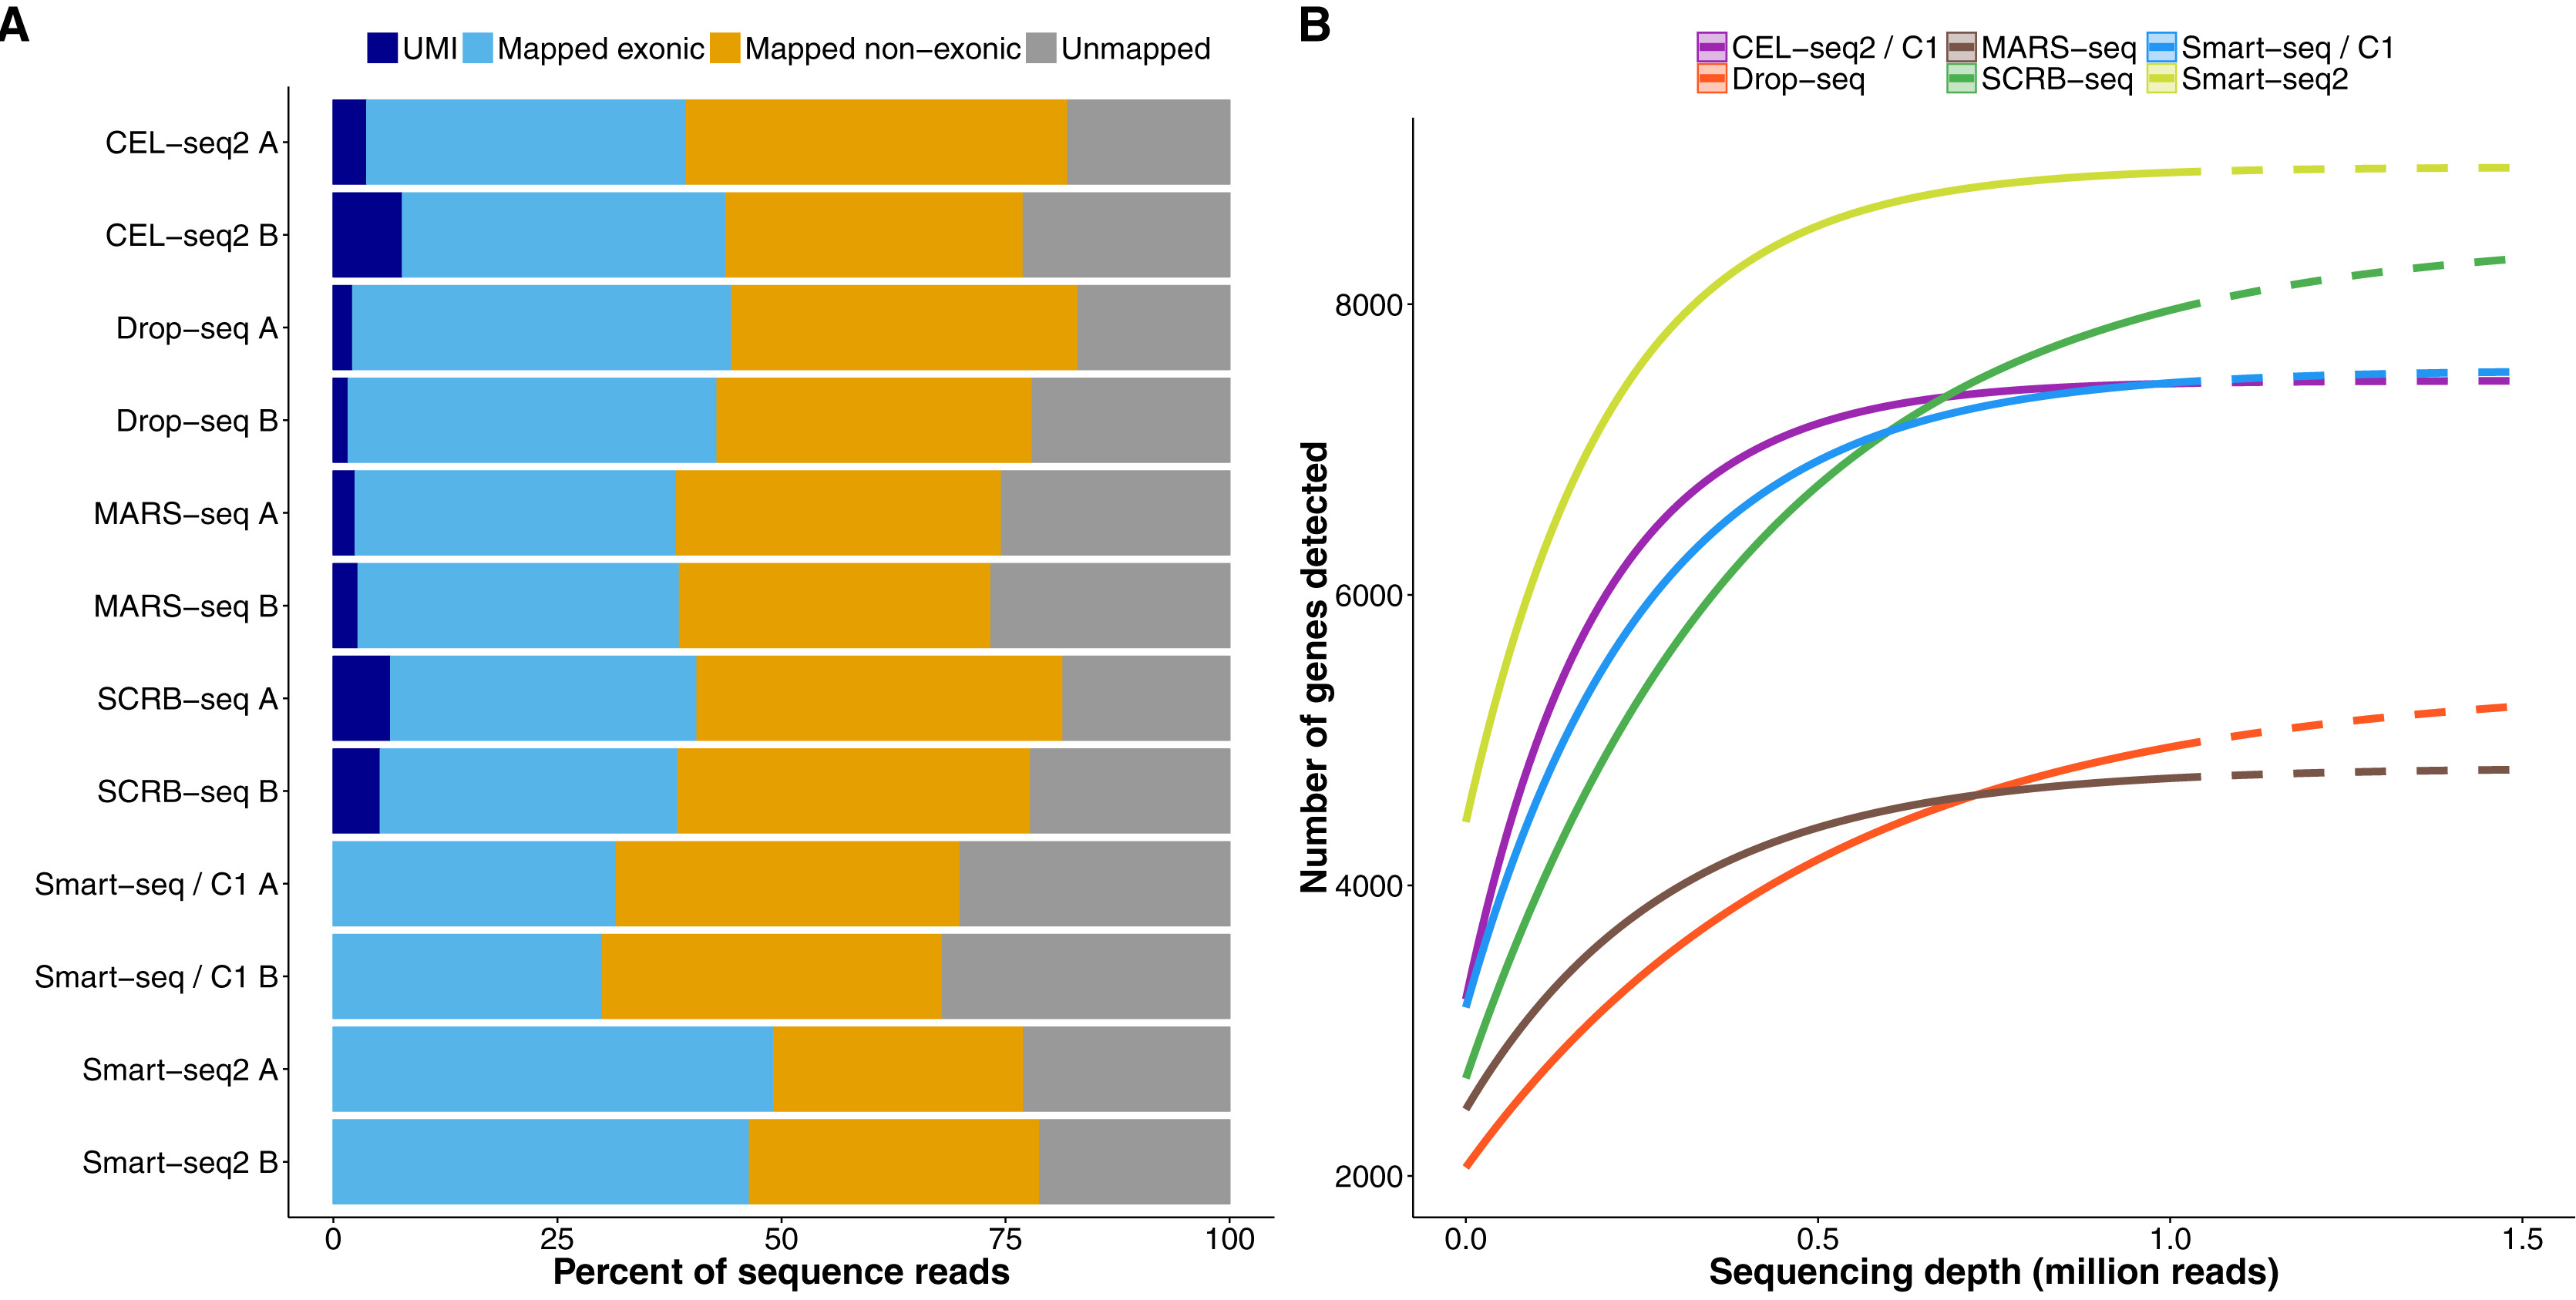
\includegraphics[width=0.95\linewidth]{scRNA_seq_comparison}
	\caption[]{Comparison of quality metrics between different scRNA-seq technologies. (a) Fraction of reads mapped to exons (cyan), outside exons (orange) and unmapped (gray). -A and -B denote different replicates. For UMI methods, also shown is the fraction of reads mapping to unique UMIs (dark blue). (B) Median number of genes detected per cell (more than one count) as a function of the (downsampled) sequencing depth. Dashed lines represent extrapolated fits assuming a saturating model. Figure reprinted from \cite{Ziegenhain2017} }
	\label{fig:scRNA_seq_comparison}
\end{figure}


\subsection{Single-cell sequencing of the epigenome}

While the large majority of single-cell studies are focused on the RNA expression, transcriptomic measurements capture a single dimension of cellular heterogeneity and hence contain limited information to characterise the molecular determinants of phenotypic variation \cite{Ritchie2015}. Consequently, gene expression markers have been identified for a myriad of biological systems, but the accompanying epigenetic changes and the role of other molecular layers in driving cell fate decisions remains poorly understood \cite{Griffiths2018,Kelsey2017,Bheda2014}.

\subsubsection{DNA methylation} \label{section:dna_methylation}
DNA methylation is a stable epigenetic modification that is strongly associated with transcriptional regulation and lineage diversification in both developmental and adult tissues \cite{Jin2018, Harrison2011, Lee2014, Smith2013}. Its classical roles include the silencing of repeating elements, inactivation of the X chromosome, gene imprinting, and repression of gene expression \cite{Jones2012}. Consistently, the disruption of the DNA methylation machinery is associated with multiple dysfunctions, including cancer \cite{Baylin2011}, autoimmune diseases \cite{Liu2013} and neurological disorders \cite{Amir1999}.\\
In mammalian genomes, DNA methylation predominantly occurs at CpG dinucleotides (mCG). The presence of DNA methylation in non-CpG cntexts (mCH) has been confirmed, albeit its functional role remains controverisal \cite{He2015, Ramsahoye2000, Lister2009}.\\
% The establishment of DNA methylation signatures begin during development by the interplay of \textit{de novo} methylation and demethylation events. In mammals, methylation events are orchestrated by three different DNA methyltransferase enzymes with similar structure but different activity patterns: Dnmt1, Dnmt3a, Dnmt3b.
% Dnmt1 binds hemi-methylated cytosines and is responsible for the maintenance of DNA methylation in replicating cells. In contrast, Dnmt3a and Dnmt3b are known as the de novo methyltransferases and are responsible for establishing the DNA methylation profiles in early development.

Alongisde developments in scRNA-seq technologies, protocols for the profiling of DNA methylation at the single-cell level also emerged from its bulk counterparts (\Cref{fig:methylation_protocols}), notably bisulfite sequencing (BS-seq) \cite{Smallwood2014,Guo2013,Gravina2016,Farlik2015}. The underlying principle of BS-seq is the treatment of the DNA with sodium bisulfite before DNA sequencing, which converts unmethylated cytosine residues to uracil (and eventually to thymine, after PCR amplification), leaving 5-methylcytosine residues intact. The resulting C$\to$T transitions are detected by DNA sequencing, thereby yelding DNA methylation information at the single-nucleotide resolution \cite{Frommer1992,Clark2016,Clark2017}.\\

\begin{figure}[H]
	\centering
	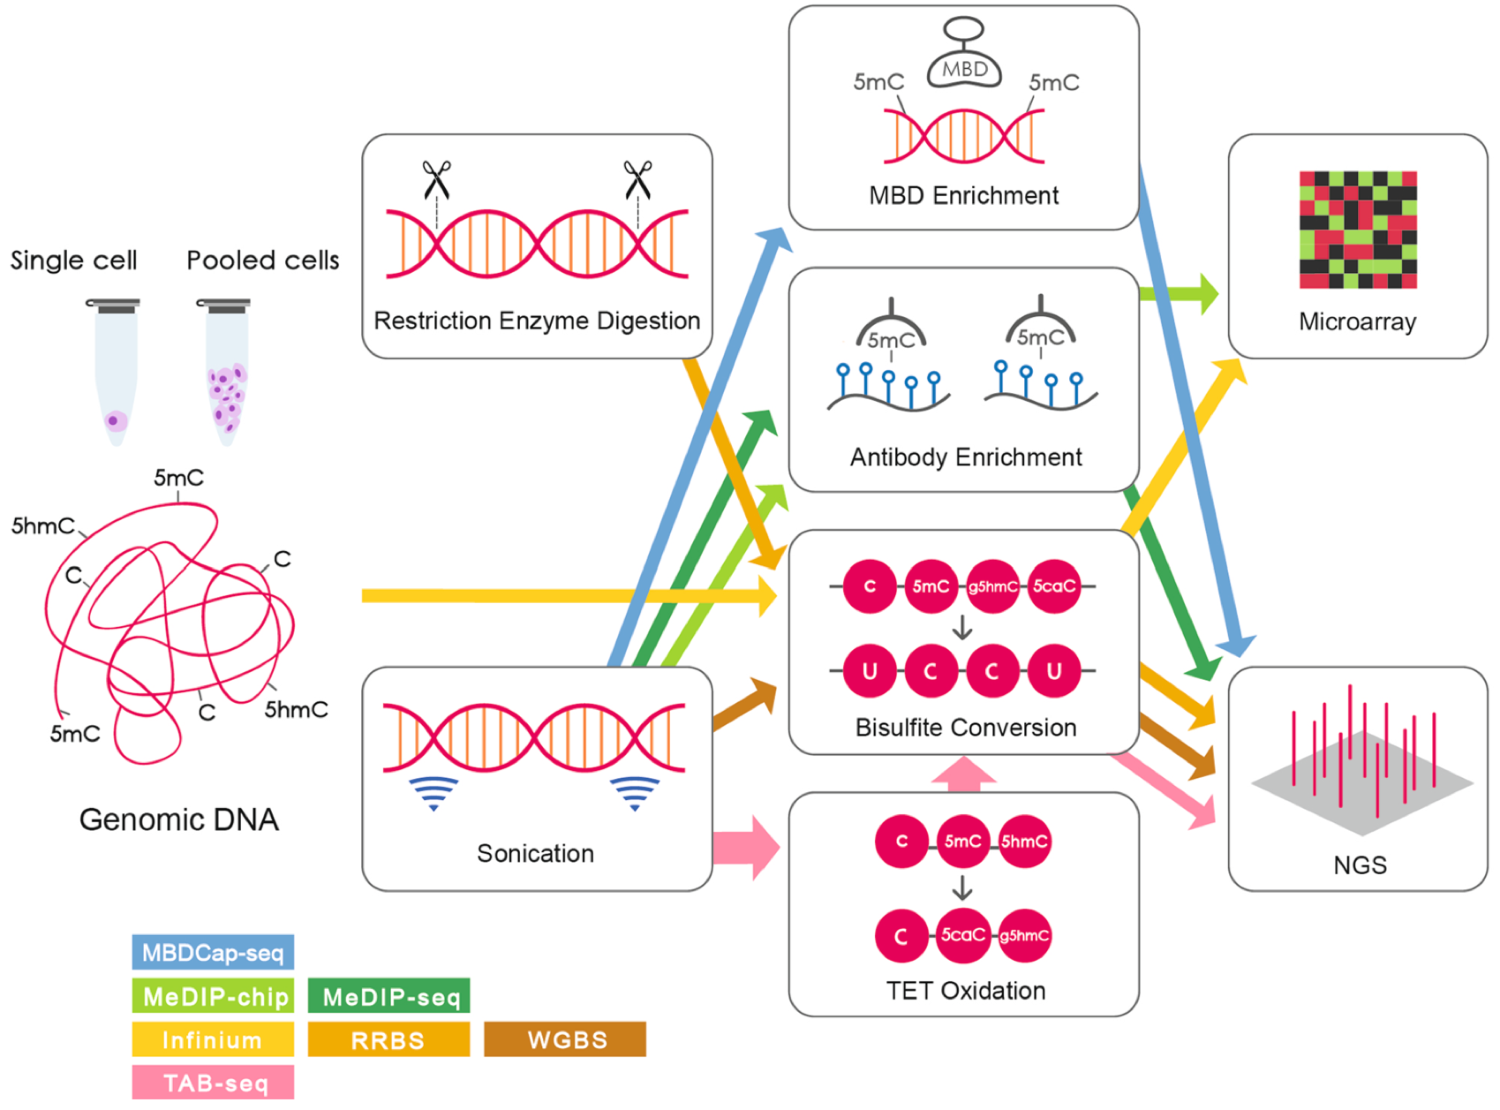
\includegraphics[width=0.8\linewidth]{methylation_protocols}
	\caption[]{Workflow of DNA methylation profiling protocols. Reprinted from \cite{Yong2016}}
	\label{fig:methylation_protocols}
\end{figure}

Nevertheless, the high degree of DNA degradation caused by the purification steps and the bisulfite treatment impaired the use of conventional BS-seq with low starting amounts of DNA. To address this problem, \cite{Smallwood2014} adapted the post-bisulfite adaptor tagging (PBAT) protocol with multiple rounds of 3' random primer amplification (\Cref{fig:scBS}). When the bisulfite treatment is performed before ligation of adaptors, rather than afterwards, loss o adapter-tagged molecules is minimised, hence enabling the use of scBS-seq with little input material.\\

In a proof of concept study, \cite{Smallwood2014} applied scBS-seq on ovulated metaphase II oocytes (MIIs) and mouse ESCs. They reported an average coverage of 3.7 million CpG dinucleotides (17.7\%) per cell and revealed extensive heterogeneity in the methylome of pluripotent cells. \\

\begin{figure}[H]
	\centering
	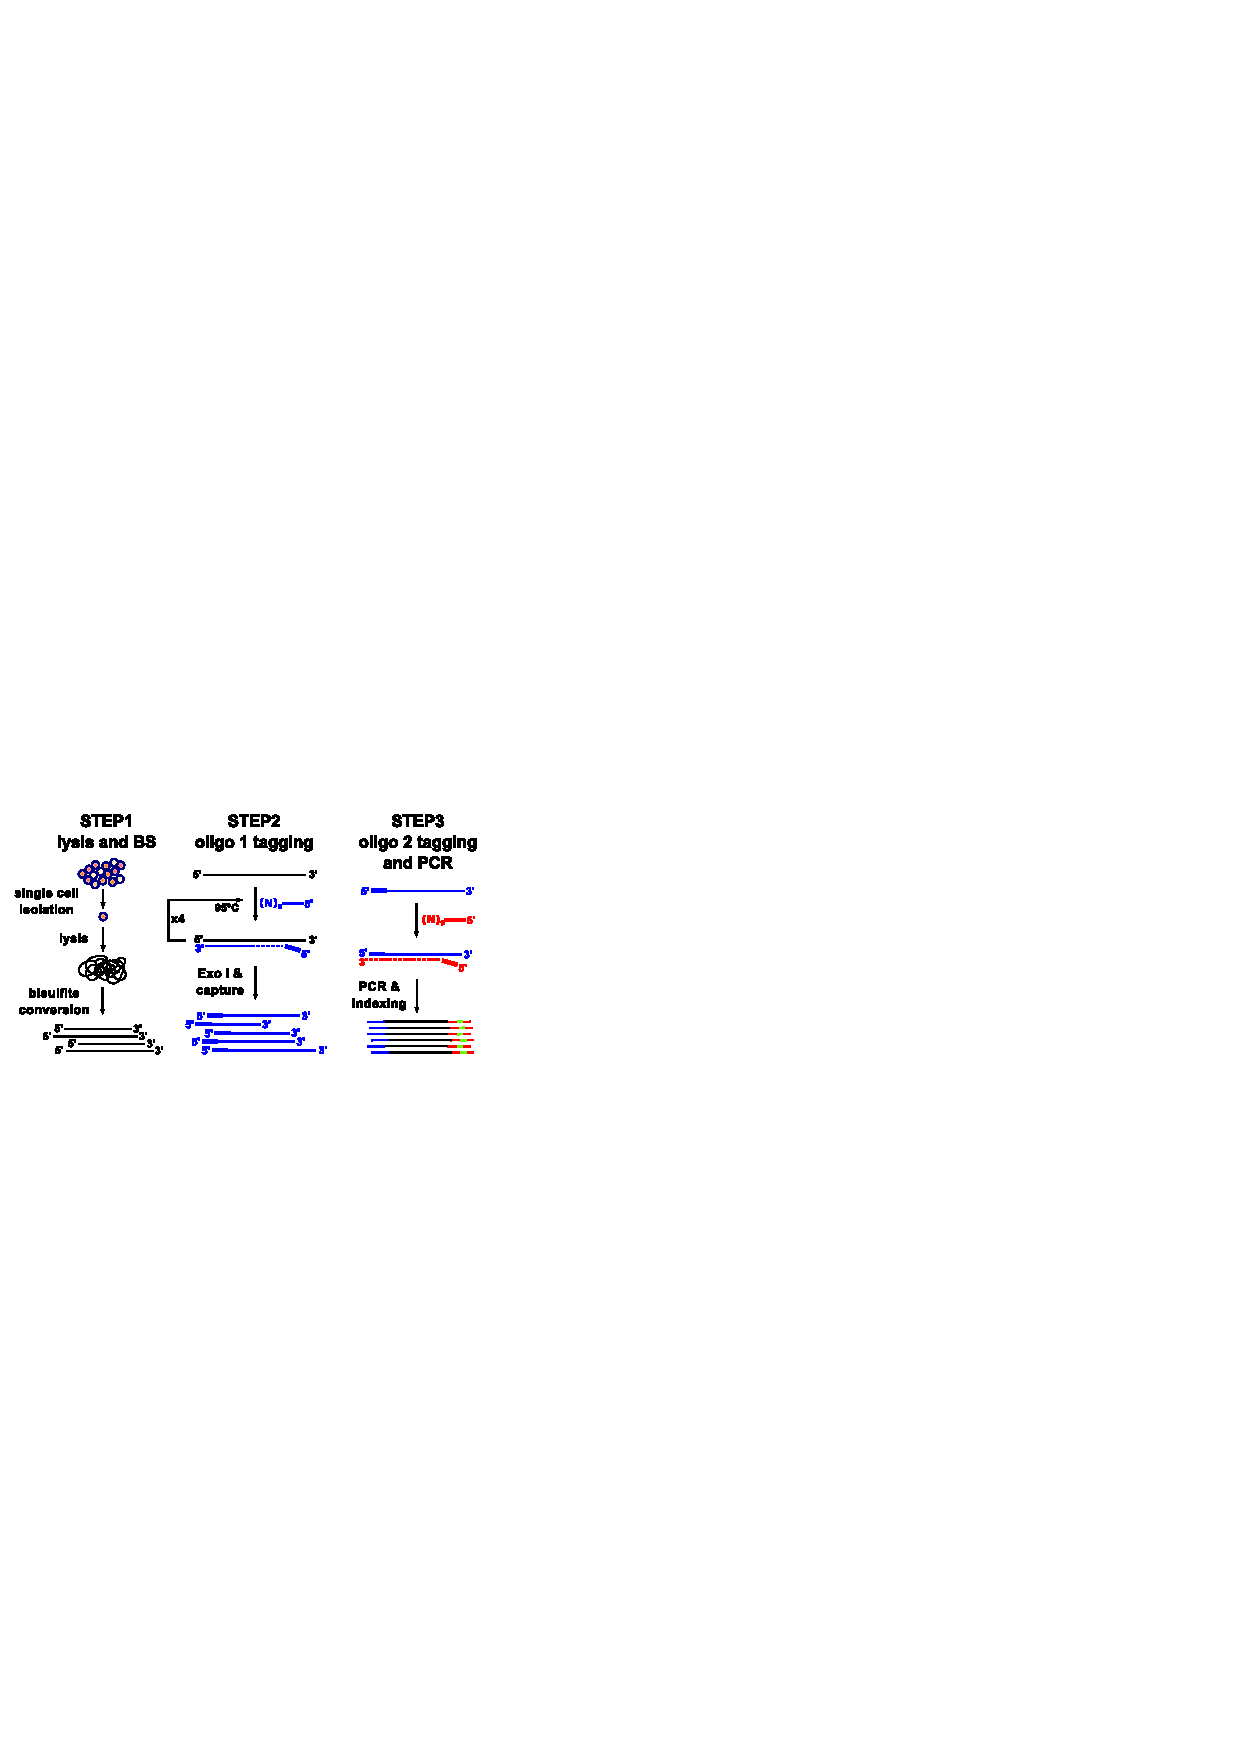
\includegraphics[width=0.8\linewidth]{scBS_protocol}
	\caption[]{scBS-seq profiling protocol. In the first step, cells are isolated and lysed, followed by bisulfite conversion. In the second step, five round of random priming amplification are performed using the first sequencing adaptor. In the third step, this process is repeated using the second sequencing adaptor. Finally, the resulting fragments are PCR-amplified and sequenced. Figure reprinted from \cite{Smallwood2014}.}
	\label{fig:scBS}
\end{figure}

Alongside scBS, other bulk sequencing methods were also adapted to the single cell resolution, with different trade-offs between coverage and costs. For instance, \cite{Guo2015} adapted the reduced-representation bisulfite sequencing (RRBS-seq) to low starting material by integrating all experimental steps before PCR amplification into a single tube. The key principle behind RRBB-seq is to digest the DNA with a restriction endonuclease, followed by a size-selection strategy to enrich for CpG-dense areas \cite{Meissner2005}. This approach significantly reduces sequencing costs at the expense of low coverage in CpG-poor genomic areas, which include repetitive elements, gene bodies and enhancer elements \cite{Martin-Herranz2017}.\\

(IMPROVE) More recently, combinatorial indexing technologies such as sci-MET \cite{Mulqueen2018} and snmC-seq \cite{Luo2018} enabled the profiling of thousands of single cells in parallel, increasing the highthroughput, albeit yelding lower coverage than scBS.seq (maximum of 7.0\% observed CpG sites) \cite{Mulqueen2018}.
	%However, the scWGBS protocol processes each cell in its own reaction vessel, severely limiting cell count throughput. Furthermore, align- ment rates for traditional scWGBS libraries are much lower (on the order of 25 􏰀 20%) than for the equivalent bulk protocol3–7, which increases the cost of obtaining sufficient information
	%In this platform, DNA (or RNA) within nuclei or cells is modified with an indexed adap- tor corresponding to one of 96 (or 384) wells while nuclear integ- rity is maintained
	%such that the probability of two nuclei harboring the same initial index ending up in the same well is low
	 % PCR is then used to incorporate a second index and generate a cell-specific barcode composed of the unique index combinations
	% using transposomes with adaptors depleted of cytosines, and thus unaffected by bisulfite treatment
	% 3). Overall, this preparation produced a mean alignment rate of 59.9 􏰀 11.9%. In total, 285 cells met a read depth threshold of 30,000 uniquely aligned reads (mean 186,710) and were carried through subse- quent analysis, with the percent of CGs covered genome-wide ranging from 0.10% to 4.5% (mean 0.82 􏰀 0.85%; 

\subsubsection{Chromatin accessibility} \label{section:chromatin_accessibility}
In eukaryotes, the genome is packed into a compact complex of DNA, RNA and proteins called chromatin. Several layers of chromatin condensation have been identified, the fundamental unit being the nucleosome, which consists on a string of \~ 150bp of DNA wrapped around histone proteins, with linker DNA of \~ 80bp connecting them \cite{Klemm2019,Tsompana2014}. The N-terminal tails of the histones emerge from the nucleosome and are a strong hotspot for chemical modifications, including methylation, acetylation, phosphorylation and others \cite{Bannister2011}. The complex interaction between a histone modification and the corresponding position, often called the histone code, is an important driver of epigenetic regulation and an active area of research \cite{Zhao2015}. \\
In addition to the histone modifications, the positioning of the nucleosomes provide another layer of gene expression regulation, mostly by exposing or sheltering transcription factors binding sites \cite{Jiang2009}. In general, active regulatory regions tend to have low occupancy of nucleosomes, whereas inactive regions show a high density of nucleosomes \cite{Struhl2013}. Thus, the profiling of DNA accessibility and transcription factor footprints represents an important dimension to understand the regulation of gene expression.\\

Traditionally, four main experimental approaches have been used to map chromatin accessibility in a genome-wide and high-throughput manner: MNase sequencing (MNase-seq) \cite{Kaplan2008}, DNase sequencing (DNase-seq) \cite{Song2010}, transposase-accessible chromatin followed by sequencing (ATAC-seq) \cite{Buenrostro2013} and Nucleosome Occupancy and Methylome-sequencing (NOMe-seq) \cite{Kelly2012}. A systematic comparison with a controlled experimental design can be found in \cite{Nordstrom2019}.

In MNase-seq, the chromatin is incubated with a micrococcal nuclease (MNase), an enzyme that degrades naked DNA, followed by purification, PCR amplification and next-generation sequencing. As nucleosomes protect the DNA from digestion, the resulting sequencing fragments reveal nucleosome location, hence providing an inverse measure of chromatin accessibility \cite{Kaplan2008}.\\

In DNase-seq, the chromatin is incubated with DNAse, an enzyme that in low concentrations cuts nucleosome-free regions. Hence accessible sites, typically called DNase I hyper-sensitive sites, are released and sequenced \cite{Song2010}. In contrast to MNase-seq, this assay provides a direct measure of chromatin accessibility, and became one of the gold standards to map chromatin accessibility in the human genome by the ENCODE consortium \cite{ENCODE2012,Thurman2012}. However, it has been reported that DNase I introduces significant cleaveage biases, thus affecting its reliability to infer transcription factor footprints \cite{He2013}.\\

In ATAC-seq, the chromatin is incubated with hyperactive mutant Tn5 transposase, an enzyme that inserts artifical sequencing adapters into nucleosome-free regions. Subsequently, the adaptors are purified, PCR-amplified  and sequenced. As in DNase-seq, it provides a direct measure of chromatin accessibility. Yet, in the last years it has arguably displaced DNase-seq or MNase-seq as the \textit{de facto} method for profiling chromatin accessibility due to its fast and sensitive protocol \cite{Buenrostro2015b,Tsompana2014,Nordstrom2019}.\\

NOME-seq follows a very different strategy than the previous technologies. The idea is to incubate cells with a GpC methyltransferase (M.CviPI), which labels accessible (or nucleosome depleted) GpC sites by DNA methylation. In mammalian genomes, cytosine residues in GpC dinucleotides are methylated at a very low rate \cite{Kilgore2007}. Hence, after M.CviPI treatment and bisulfite sequencing, GpC methylation marks can be interpreted as direct read outs for chromatin accessibility, as opposed to the CpG methylation readouts, which can be interpreted as endogenous DNA methylation marks \cite{Kelly2012}.\\
NOME-seq has a range of appealing properties in comparison with count-based methods such as ATAC-seq or DNAseq-seq. First, the obvious gain of simultaneously measuring another epigenetic readout such as DNA methylation with little additional cost. Second, the resolution of the method is determined by the frequency of GpC sites within the genome (\~1 in 16 bp), rather than the size of a library fragment (usually >100 bp). This allows the robust inspection of individual regulatory elements, nucleosome positioning and transcription factor footprints \cite{Kelly2012,Pott2016,Nordstrom2019}. Third, missing data can be easily discriminated from inaccessible chromatin. Importantly, this implies that lowly accessible sites will not suffer from increased technical variation (due to low read counts) compared to highly accessible sites. Finally, the M.CviPI enzyme shows less sequence motif biases than the DNAse or the Tn5 transposase \cite{Nordstrom2019}\\ 
The downsides of the approach are the high sequencing depth requirements and the need to discard read outs from GCG positions (21\%) and CGC positions (27\%).

\begin{figure}[H]
	\centering
	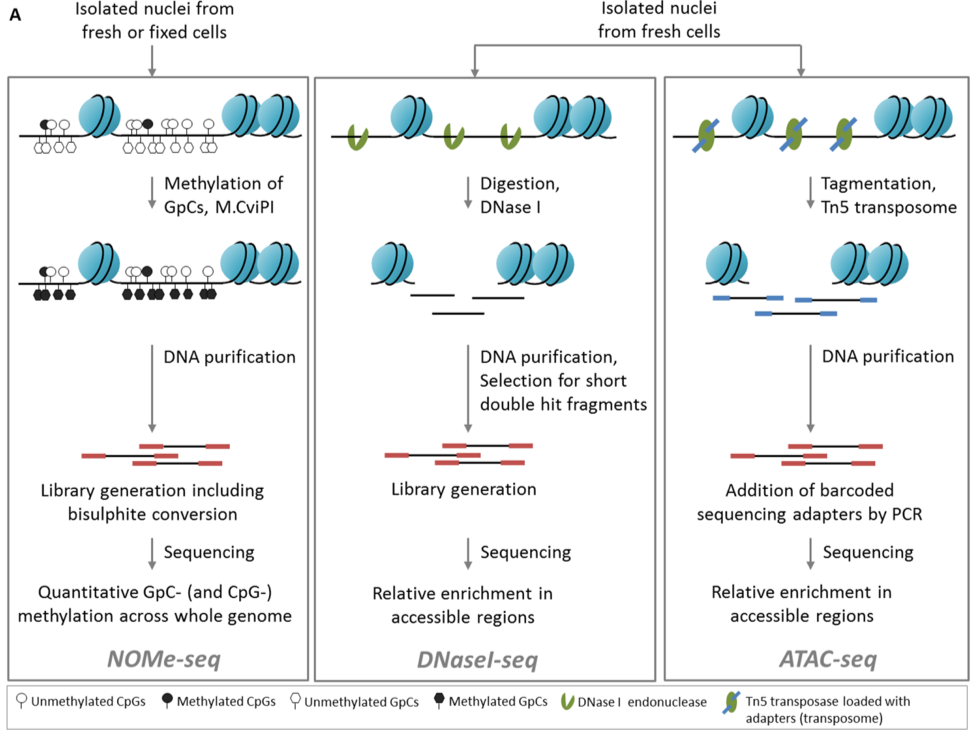
\includegraphics[width=0.9\linewidth]{ChromatinAcc_protocols}
	\caption[]{High-level workflow of the three main chromatin accessibility assays: NOME-seq, DNase-seq and ATAC-seq. Reprinted from \cite{Nordstrom2019}. }
	\label{fig:ChromatinAcc_protocols}
\end{figure}

% Figure 1. Chromatin accessibility assays. A. NOMe-seq (left): Isolated nuclei are treated with M.CviPI, which methylates cytosines in GpC- dinucleotides. The DNA is purified, subjected to library preparation including bisulfite-conversion and sequenced. The resulting data give quantitative measures of GpC- and endogenous CpG-methylation at base-pair resolution across the whole genome. DNase I-seq (middle): After isolation of nuclei, chromatin is digested with DNase I. The DNA is purified and short double hit fragments are selected, which are used for library preparation and sequencing. The obtained data represent a relative enrichment of double-hit fragments in accessible regions. ATAC- seq (right): Isolated nuclei are treated with Tn5 transposase, which is loaded with sequencing adapters. After the tagmentation of chromatin (fragmentation and tagging by the transposome), the DNA is purified, barcoded by PCR and sequenced. The data give a relative read-out of tagmented fragments across accessible regions. B. Snapshot of chromatin accessibility data relative to genomic coordinates for section of chr12. NOMe-seq (blue): Quantitative measure of GCH-methylation and NDRs called with gNOMeHMM are shown. The GCH coverage track indicates if number of reads is 5 (downward bars) or higher (upward bars). DNase I- (red) and ATAC-seq (orange): Read coverage and NDRs called with MACS2 are shown.

As with DNA methylation, single-cell profiling methods for chromatin accessibility also emerged from its bulk counterparts, including ATAC-seq\cite{Buenrostro2015a}, NOME-seq \cite{Pott2016} and DNase-seq \cite{Jin2015}.
\\

Due to its cost-effective strategy, single-cell ATAC-seq has become the most established technique to map open chromatin regions, revealing extensive heterogeneity across different cellular populations \cite{Cusanovich2015,Cao2018,Chen2018}. 

Compared to bulk ATAC-seq, scATAC-seq libraries are notably sparse. In a satured library, \cite{Cusanovich2015} reported a range of \~ 500 to \~ 70,000 mapped reads per cell, with a median of 2503. This represents less than 25\% of the molecular complexity expected from 500-cell bulk experiments. Yet, despite the low coverage, they showed that cell-type mixtures can be confidently deconvoluted. Later, in a pioneer effort, \cite{Cusanovich2018b} generated an atlas of chromatin accessibiliy for different mouse tissues, defining the first \textit{in vivo} landscape of the regulatory genome single-cell resolution.\\

However, the sparse nature of scATAC-seq makes it impractical for the study of heterogeneity in individual regulatory elements. This is addressed mostly by NOME-seq, which at the expensive of more expensive sequencing and limited scalability, it provides base-pair resolution readouts, even at the single cell resolution \cite{Pott2016}.


\subsection{Multi-modal single-cell sequencing}
Cellular phenotypes have been historically characterised using exploratory methods in single molecular layers, most commonly the transcriptome. However, phenotypes result from the combination of multiple sources of biological information, including the genetic background, epigenetic marks, protein levels or lipid composition. Undoubtedly, no single "-omics" technology can capture the intricacy of complex molecular mechanisms, but the collective information has the potential to draw a more comprehensive picture of biological processses as well as clinically relevant traits \cite{Hasin2017,Ritchie2015}.\\
Motivated by this assumption, multiple omics are being increasingly applied across a wide range of biological domains, including cancer biology \cite{Akavia2010,Gerstung2015}, regulatory genomics \cite{Chen2016}, microbiology \cite{Kim2016} or host-pathogen interactions \cite{Soderholm2016}.\\ 

Recent technological advances have enabled the profiling of multiple omics in the same single cell, which has the potential to provide a more comprehensive understanding of biological processess, including mechanistic relationships between the (epi)genome and the transcriptome.\\
Multi-modal sequencing technologies are becoming rapidly available and its explosion is likely to mirror the trend of scRNA-seq technologies. As reviewed in \cite{Stuart2019,Chappell2018}, multi-modal measurements can be obtained using four broad strategies:
\begin{itemize}
	
	\item \textbf{Application of a non-destructive assay before a destructive one}: the most prominent example is multiparameter fluorescence-activated cell sorting (FACS) followed by destructive high-throughput sequencing \cite{Paul2015}. Although simple and efficient, this approach requires prior knowledge of gene expression markers to sort the populations of interest and is limited by the spectral overlap of fluorescence reporters.

	\item \textbf{Physical isolation of different cellular fractions followed by independent high-throughput sequencing}: this technique was pioneered with the simultaneous genome and transcriptome sequencing (G\&T-seq) \cite{Macaulay2015}. After cell lysis, the mRNA fraction is separated from the genomic DNA fraction using biotinylated or paramagnetic oligo(dT) beads, followed by conventional uni-modal sequencing of the mRNA and the DNA. This strategy allows the simultaneous profiling of transcriptomic measurements with genome-derived measurements, including DNA sequence, copy number variation, DNA methylation or chromatin accessibility \cite{Macaulay2015,Hou2016,Angermueller2016,Hu2016}\\
	A clear advantage of this methodology is its unsupervised nature, which makes it particularly useful for the study of tissues with complex heterogeneity.
		%TO-DO: SCI-CAR

	\item \textbf{Conversion of different molecular layers to a common format that can be simultaneously measured using the same readout}: this represents a powerful methodology, as it allows multiple modalities to be profiled in a single workflow. Prominent examples are the simultaneous measure of surface proteins and mRNA expression as in Cellular indexing of transcriptomes and epitopes by sequencing (CITE-seq\cite{Stoeckius2017}) and RNA expression and protein sequencing assay (REAP-seq\cite{Peterson2017}). The idea is to incubate cells with antibodies tagged with oligonucleotides that target specific proteins. Subsequently, additional barcodes are introduced for PCR amplification and a poly(A)-tail selection step is performed, allowing the simultaneous pooling of mRNAs (cDNAs) and antibody tags. Finally, After PCR amplification, both types of molecules can be separated by size and sequenced.\\
	In practice, this principle is significantly more powerful than FACS, as the DNA barcodes can be resolved with very high sensitivity by sequencing and their complexity is limited by the number of nucleotides ($4^N$ where $N$ is the length of the barcode)\\
	A second prominent example is NOME-seq, described in \Cref{section:chromatin_accessibility}. By labelling accessibile GpC sites with DNA methylation marks, one can simultaneously measure endogenous DNA methylation and chromatin accessibility using a single bisulfite sequencing assay.
\end{itemize}
	
Combinations of the three approaches above have also been achieved. One of them, single-cell nucleosome, methylome and transcriptome (scNMT-seq\cite{Clark2018}), which is presented in this thesis, combines the principle of physical isolation with the conversion to a common format to achieve a simultaneous measurement of three molecular layers.\\

(IMPROVE) Although they have been proven successful, single-cell multiomics approaches still face numerous difficulties, both from the experimental and the computational side. Single-cell approaches yield outputs with low coverage and high levels of technical noise, which generally gets exacerbated when profiling multiple omics. A clear example is scNMT-seq, where an almost \%50 decrease of coverage is observed in DNA methylation with respect to scM\&T-seq. Similarly, chromatin accessible measurements in sci-CAR showed \~10-fold less complexity than scATAC-seq. Additionally, most single-cell multi-modal technologies remain more expensive and less scalable than the uni-modal counterparts. Yet, due to intrisic high levels of technical noise and missing values, the profiling of large number of cells is required for the extraction of biologically meaningful conclusions.

